%%%%%%%%%%%%%%%%%%%%%%%%%%%%%%%%%%%%%%%%%%%%%%%%%%%%%%%%%%%%%%%%%%%%%%%%%%%%%%%%%%%%%%%
%%%%%%%%%%%%%%%%%%%%%%%%%%%%%%%%%%%%%%%%%%%%%%%%%%%%%%%%%%%%%%%%%%%%%%%%%%%%%%%%%%%%%%%
%%%%%%%%%%%%%%%%%%%%%%%%%%%%%%%%%%%%%%%%%%%%%%%%%%%%%%%%%%%%%%%%%%%%%%%%%%%%%%%%%%%%%%%
\section{ Matrizes definidas positivas}

\index{Matriz!Definida positiva}

%%%%%%%%%%%%%%%%%%%%%%%%%%%%%%%%%%%%%%%%%%%%%%%%%%%%%%%%%%%%%%%%%%%%%%%%%%%%%%%%
\begin{definition}[Matriz definida positiva:]\label{def:positivematrix0}
Conhecida uma matriz quadrada $\MATRIX{A} \in \mathbb{R}^{N \times N}$. 
\begin{itemize}
\item Esta é definida positiva, se para todo vetor não nulo $\VECTOR{x} \in \mathbb{R}^N$
se cumpre que \cite[pp. 159]{golub2013matrix} 
\begin{equation}
\VECTOR{x}^{\transpose} \MATRIX{A} \VECTOR{x} > 0.
\end{equation}
\end{itemize}
\end{definition}




%%%%%%%%%%%%%%%%%%%%%%%%%%%%%%%%%%%%%%%%%%%%%%%%%%%%%%%%%%%%%%%%%%%%%%%%%%%%%%%%
\begin{theorem}[Autovalores positivos e matrizes definidas positivas:]\label{theo:positivematrix1}
Conhecida uma matriz quadrada $\MATRIX{A} \in \mathbb{R}^{N \times N}$, com  autovalores $\lambda_n$,
e autovetores $\VECTOR{e}_n$, $\forall n \in \{1, 2, ..., N\}$.
\begin{itemize}
\item Se $\MATRIX{A}$ é uma matriz definida positiva, então\footnote{\label{foot:theo:positivematrix1}A
demonstração pode ser vista na Prova \ref{proof:theo:positivematrix1}.}  
podemos afirmar que todos os autovalores 
\begin{equation}
\lambda_n > 0.
\end{equation}
\item Se todos os autovalores $\lambda_n$ são positivos e a matriz $\MATRIX{A}$ é \hyperref[def:symmetricmatrix0]{simétrica},
\begin{equation}
\lambda_n > 0 \qquad \wedge \qquad \MATRIX{A}=\MATRIX{A}^{\transpose},
\end{equation}
 então\footnote{A
demonstração pode ser vista na Prova \ref{proof:theo:positivematrix2}.} 
podemos afirmar que $\MATRIX{A}$ é uma matriz definida positiva.
\end{itemize}
\end{theorem}

\begin{tcbattention}
Conhecida uma matriz quadrada $\MATRIX{A} \in \mathbb{R}^{N \times N}$, 
com  autovalores $\lambda_n$, $\forall n \in \{1, 2, ..., N\}$.
\begin{itemize}
\item Que todos os autovalores $\lambda_n$ sejam positivos não garante que a matriz $\MATRIX{A}$
seja definida positiva. Para mais detalhes, ver o Exemplo \ref{ex:positivematrix1}.
\end{itemize}
\end{tcbattention}

%%%%%%%%%%%%%%%%%%%%%%%%%%%%%%%%%%%%%%%%%%%%%%%%%%%%%%%%%%%%%%%%%%%%%%%%%%%%%%%%
\noindent
\begin{minipage}{0.5\textwidth}
\begin{example}[Autovalores positivos não garantem matrizes definidas positivas:]
\label{ex:positivematrix1}
Conhecida uma matriz quadrada $\MATRIX{A}$ com autovalores positivos agrupados no vetor $\VECTOR{\lambda}_{\VECTOR{a}}$, 
\begin{equation}
\MATRIX{A}=
\begin{bmatrix}
1 & -8\\
0 & 2
\end{bmatrix}
\quad \rightarrow \quad 
\VECTOR{\lambda}_{\VECTOR{a}}=
\begin{bmatrix}
1 \\
2
\end{bmatrix}.
\end{equation}
Podemos verificar que a matriz $\MATRIX{A}$ não é definida positiva,
\begin{equation}
\VECTOR{x}=
\begin{bmatrix}
1 \\
1
\end{bmatrix}
\quad \rightarrow \quad 
-5 = \VECTOR{x}^{\transpose}\MATRIX{A}\VECTOR{x}<0.
\end{equation}
A superfície $\VECTOR{x}^{\transpose}\MATRIX{A}\VECTOR{x}$ 
pode ser vista na Figura \ref{fig:ex:positivematrix1}.
\end{example}
\end{minipage}
\begin{minipage}{0.5\textwidth}
     \begin{figure}[H]
         \centering
         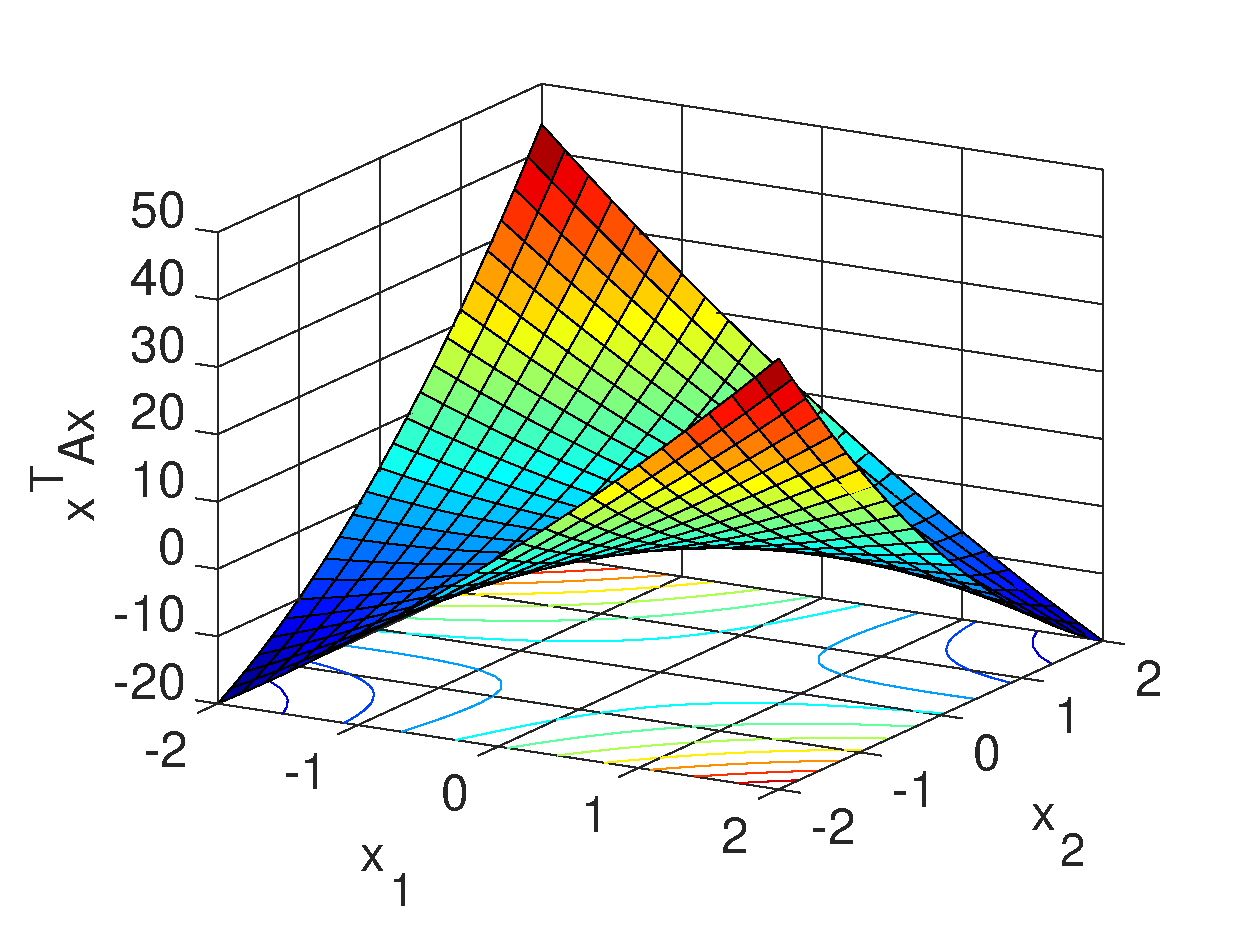
\includegraphics[width=0.98\textwidth]{chapters/teoria-basica/mfiles/positive-matrix/surfcexAx.eps}
         \caption{Superfície $\VECTOR{x}^{\transpose}\MATRIX{A}\VECTOR{x}$. }
         \label{fig:ex:positivematrix1}
     \end{figure}
\end{minipage}

%%%%%%%%%%%%%%%%%%%%%%%%%%%%%%%%%%%%%%%%%%%%%%%%%%%%%%%%%%%%%%%%%%%%%%%%%%%%%%%%
\begin{theorem}[Matriz inversa e matrizes definidas positivas:]\label{theo:positivematrix:2}
Conhecida uma matriz  $\MATRIX{A} \in \mathbb{R}^{N \times N}$, com  autovalores $\lambda_n$,
$\forall n \in \{1, 2, ..., N\}$.
\begin{itemize}
\item Se $\MATRIX{A}$ é uma matriz simétrica e definida positiva, então\footnote{A
demonstração pode ser vista na Prova \ref{proof:theo:positivematrix:2}.}  
a matriz $\MATRIX{A}^{-1}$ tambem é definida positiva.
\end{itemize}
\end{theorem}

